\documentclass[a4j]{jarticle}

\usepackage[dvipdfmx]{graphicx}
\usepackage{url}
\usepackage{here}
\usepackage{listings}
\usepackage{amsmath,amssymb}
\usepackage[dvipdfmx]{color}

\setlength{\headsep}{-5mm}
\setlength{\oddsidemargin}{0mm}
\setlength{\textwidth}{165mm}
\setlength{\textheight}{230mm}
\setlength{\footskip}{20mm}

\title{
\vspace{30mm}
{\bf 子育て支援システム}
\\
\vspace{5mm}
{\bf 外部設計書v1\\
}
\vspace{120mm}
}

\author{
\vspace{5mm}
チーム名 007\\
\vspace{5mm}
}


\begin{document}
\maketitle
\tableofcontents
\newpage

\section{はじめに}
本書では弊社がシステム提案書で提案した子育て支援システムの詳細を示しています。

まず、本システムの概要及びシステムを構成するサブシステムについて示します。
次に本システムのユーザインタフェースについて示し、最後に本システムを構築するデータテーブル設計に
ついて示します。

\section{システム概要}
本システムは機能としてゲーム機能、成長記録機能、子育て窓口機能、設定機能の4つを実装します。この章では、各機能の説明及び各機能を構成するサブシステムを示します。サブシステムの詳細は第3章にて説明します。

\subsection{成長記録機能}
成長記録機能では、日々の子供の成長を記録できる機能を提供します。成長記録は日付ごとに分けて記録され、いつでも見返すことができます。他のSNSに記録を共有することもできます。
\subsubsection*{構成サブシステム}
\noindent カメラ撮影サブシステム、コメント記録サブシステム、ゲーム結果取得サブシステム、カレンダーサブシステム、共有サブシステム

\subsection{ゲーム機能}
ゲーム機能では、2〜5歳を対象とした簡単な知育ゲームを提供します。お絵描きとおつかいのゲームがあり、お絵描きではゲームの記録を成長記録機能に保存することが可能です。
\subsubsection*{構築サブシステム}
\noindent ペイントサブシステム、おつかいサブシステム、ゲーム記録保存サブシステム

\subsection{子育て窓口機能}
子育て窓口機能では、子育てに関する質問を投稿・回答することができる機能を提供します。質問の検索も可能です。
\subsubsection*{構築サブシステム}
\noindent 検索サブシステム、並び替えサブシステム、投稿サブシステム、回答サブシステム

\subsection{設定機能}
本システムの機能の1つである子育て窓口機能を利用するためには、アカウント登録を行う必要があります。設定機能では、アカウントの登録、変更、削除を行うことができます。本システムを初めて利用する場合は、設定機能において初期設定を行うところから始まります。
\subsubsection*{構成サブシステム}
\noindent アカウント登録サブシステム、登録情報変更サブシステム



%サブシステム%
\newpage
\section{サブシステム概要}
第2章で述べている4つの機能を構成しているサブシステムについて説明します。

\subsection{成長記録機能}
\subsubsection*{カメラ撮影サブシステム}
利用端末に搭載されているカメラをシステム内から起動し、写真を撮影することができます。
\subsubsection*{コメント記録サブシステム}
保存されている成長記録(写真、ゲームの結果)に対してコメントを記述することができます。成長記録を見ながらコメントを読み返すことにより、過去の思い出が振り返りやすくなります。
\subsubsection*{ゲーム結果取得サブシステム}
ゲーム機能で子供が遊んだ結果を成長記録として保存することができます。
\subsubsection*{カレンダーサブシステム}
成長記録を日付ごとに分けるサブシステムです。本システムの利用者は、画面に表示される写真を選択することによって、保存された成長記録を確認することができます。
\subsubsection*{共有サブシステム}
成長記録を他のSNSアプリケーションで共有することができます。しかし、個人が特定されるような写真の共有は推奨しません。

\subsection{ゲーム機能}
\subsubsection*{ペイントサブシステム}
お絵描きのゲームを提供します。お手本を見ながら同じものを描く機能と自由に描く機能を設けます。
\subsubsection*{おつかいサブシステム}
おつかいのゲームを提供します。特定の料理の材料を買うことで料理が完成するという内容です。
\subsubsection*{ゲーム記録保存サブシステム}
お絵描きの記録を保存するサブシステムです。保存されることにより成長記録機能での記録の閲覧が可能です。

\subsection{子育て窓口機能}
\subsubsection*{検索サブシステム}
質問の検索を行うサブシステムです。 質問したい内容・ワードを入力することで質問の内容・ワードに合致したものが表示されます。
\subsubsection*{並び替えサブシステム}
投稿された質問を並び替えるサブシステムです。
\subsubsection*{投稿サブシステム}
質問を投稿するサブシステムです。
\subsubsection*{回答サブシステム}
質問に回答を行うサブシステムです。

\subsection{設定機能}
\subsubsection*{アカウント登録サブシステム}
システムを初めて利用する際にアカウント登録を行います。登録する情報は、名前(ニックネーム可)と住んでいる都道府県です。
\subsubsection*{登録情報サブシステム}
登録情報の変更及びアカウントの削除を行うことができます。しかし、子育て窓口機能で投稿した内容などは削除されません。



%%ユーザインタフェース(UI)%%
\newpage
\section{ユーザインタフェース}
本章では、システムを構成するユーザインタフェースについて示します。

%初期画面%
\subsection{画面詳細}
本システムが提供するアプリケーションの画面遷移及び画面の詳細について説明します。
\subsubsection{初期設定画面}
図\ref{honjo_setup}に、アプリを初めて起動した際に表示される初期設定画面を示します。
この画面はユーザに『ニックネーム(名前)の入力』・『居住地域の選択』を行ってもらうために表示されます。
入力が完了しないと次の画面に遷移することはできません。

図\ref{honjo_setup}に示す番号と対応させる形式で、以下にその役割を示します。

\begin{figure}[H]
    \begin{center}
    \resizebox{8cm}{!}{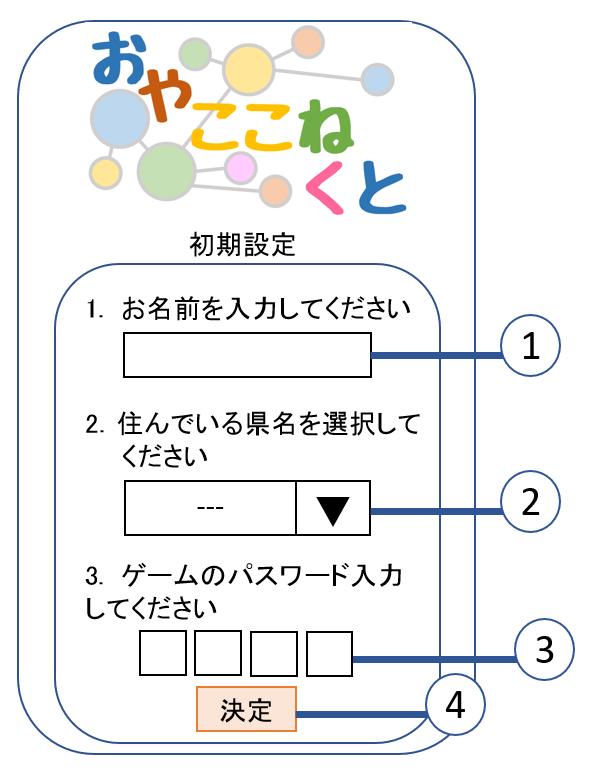
\includegraphics {honjo_FirstSetting.png}}
    \caption {初期設定画面}
    \label{honjo_setup}
    \end{center}
\end{figure}

\begin{enumerate}
  \renewcommand{\labelenumi}{\textcircled{\scriptsize \theenumi}}
  \item 名前(ニックネーム)の入力欄\\
        ユーザがアプリ内で使用したい名前を入力します。矩形領域をタップするとキーボードが開き、入力することが可能になります。
  \item 居住地域の選択欄\\
        ユーザの住んでいる地域を選択します。矩形領域をタップするとドロップダウンリストが開き、その中から住んでいる都道府県を選択します。
  \item 完了ボタン\\
        入力が完了したら押すボタンです。入力が正しくされている場合にのみメニュー画面(図\ref{honjo_main})へ遷移することができます。
\end{enumerate}


\subsubsection{メインメニュー画面}
図\ref{honjo_main}に、メインメニュー画面を示します。これは、アプリの初期設定を完了している場合に、最初に表示されます。
この画面は本アプリの持つ機能に遷移するために使用されます。

図\ref{honjo_main}に示す番号と対応させる形式で、以下にその役割を示します。

\begin{figure}[H]
    \begin{center}
    \resizebox{8cm}{!}{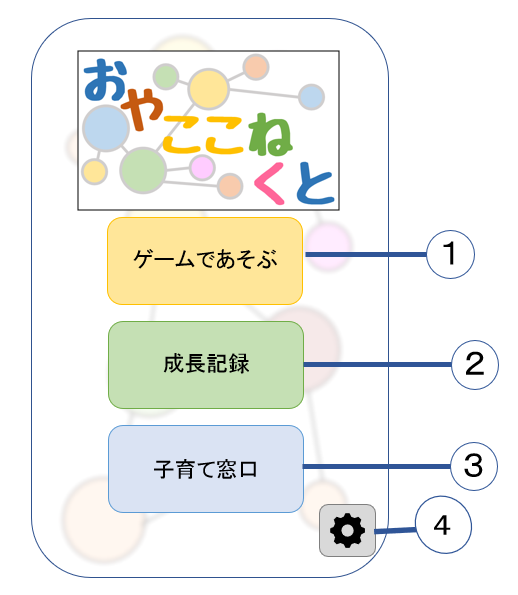
\includegraphics {honjo_main.png}}
    \caption {初期設定画面}
    \label{honjo_main}
    \end{center}
\end{figure}

\begin{enumerate}
  \renewcommand{\labelenumi}{\textcircled{\scriptsize \theenumi}}
  \item ゲーム画面遷移ボタン\\
        ゲーム機能を使用したい場合に押すボタンです。タップするとゲーム選択画面(図\ref{game})へ遷移します。
  \item 成長記録画面遷移ボタン\\
        成長記録機能を使用したい場合に押すボタンです。タップすると成長記録画面(図\ref{Grow})へ遷移します。
  \item 子育て窓口画面遷移ボタン\\
        子育て窓口機能を使用したい場合に押すボタンです。タップすると子育て窓口画面(図\ref{honjo_CR_Window})へ遷移します。
  \item 設定画面遷移ボタン\\
        アプリの設定を変更したい場合に押すボタンです。タップすると設定画面(図\ref{configuration})へ遷移します。
\end{enumerate}

%ゲーム%
\subsection{ゲーム}
図\ref{game}にゲームの画面を示します。\\
お絵描きとおつかいのゲームを提供します。

\begin{figure}[H]
    \begin{center}
    \resizebox{8cm}{!}{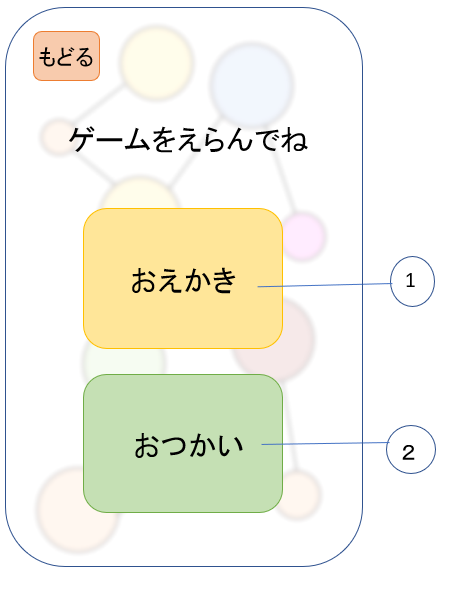
\includegraphics {game.png}}
    \caption {ゲーム画面}
    \label{game}
    \end{center}
\end{figure}

\begin{enumerate}
  \renewcommand{\labelenumi}{\textcircled{\scriptsize \theenumi}}
\item おえかき\\
  おえかきの矩形領域をタップするとお絵描きの詳細画面へ遷移します。
\item おつかい\\
  おつかいの矩形領域をタップするとおつかいのゲーム画面へ遷移します。
\end{enumerate}

\newpage
\subsubsection{おえかき}
図\ref{oekaki}におえかきの詳細画面を示します。\\
画面上のボタンをタップすることでおえかきのモードを選択することができます。\\

\begin{figure}[H]
    \begin{center}
    \resizebox{8cm}{!}{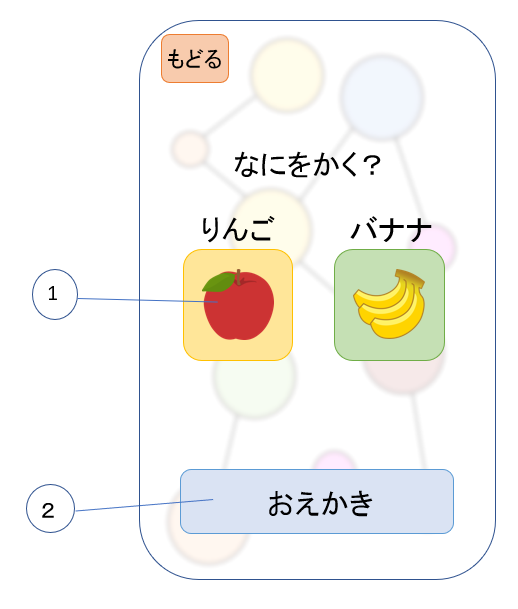
\includegraphics {oekaki.png}}
    \caption {おえかき画面}
    \label{oekaki}
    \end{center}
\end{figure}

\begin{enumerate}
  \renewcommand{\labelenumi}{\textcircled{\scriptsize \theenumi}}
\item イラストボタン\\
  イラストのボタンをタップすることで図\ref{illustration}のようにタップしたイラストを閲覧しながらのおえかきができます。
\item おえかきボタン\\
  おえかきのボタンをタップすることでおえかきの図\ref{oekaki2}のゲーム画面に遷移し、自由におえかきができます。
\end{enumerate}

\begin{figure}[H]
    \begin{center}
    \resizebox{8cm}{!}{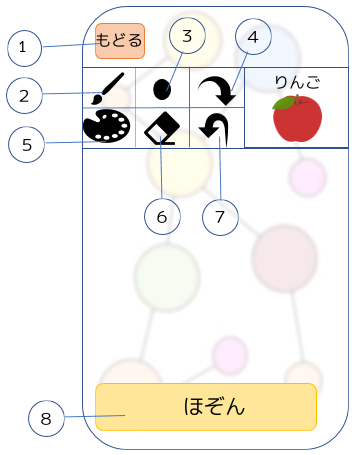
\includegraphics {illustration.png}}
    \caption {イラスト}
    \label{illustration}
    \end{center}
\end{figure}

\begin{enumerate}
  \renewcommand{\labelenumi}{\textcircled{\scriptsize \theenumi}}
\item もどるボタン\\
  もどるボタンをタップすることでおえかき画面に遷移します。
\item 保存ボタン\\
  保存ボタンをタップすることでおえかきが成長記録として保存されます。
\end{enumerate}


\begin{figure}[H]
    \begin{center}
    \resizebox{8cm}{!}{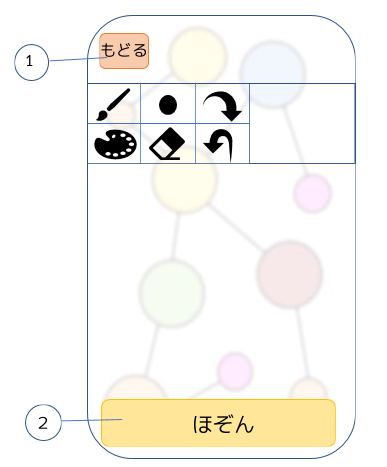
\includegraphics {oekaki2.png}}
    \caption {おえかき}
    \label{oekaki2}
    \end{center}
\end{figure}

\begin{enumerate}
  \renewcommand{\labelenumi}{\textcircled{\scriptsize \theenumi}}
\item もどるボタン\\
  もどるボタンをタップすることでおえかき画面(図\ref{oekaki2})に遷移します。
\item 保存ボタン\\
  保存ボタンをタップすることでおえかきが成長記録として保存されます。
\end{enumerate}

\newpage
\subsubsection{おつかい}
図\ref{otukai1}におつかいの詳細画面を示します。\\
おつかいは作りたい料理を選択し、その料理に必要な材料をお店から買ってくるゲームです。\\

\begin{figure}[H]
    \begin{center}
    \resizebox{8cm}{!}{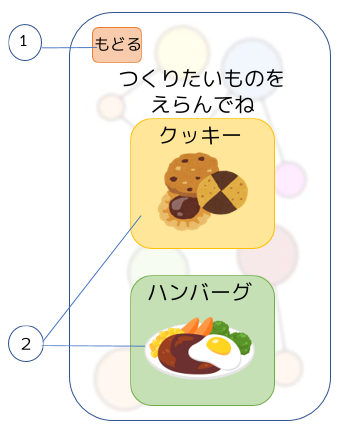
\includegraphics {otukai1.png}}
    \caption {おつかい}
    \label{otukai1}
    \end{center}
\end{figure}

\begin{enumerate}
  \renewcommand{\labelenumi}{\textcircled{\scriptsize \theenumi}}
\item もどるボタン\\
  もどるボタンをタップすることでゲーム画面(図\ref{game})に遷移します。
\item イラストボタン\\
  図\ref{otukai1}の料理のイラストボタンをタップするとその料理の材料画面(図\ref{material})に遷移します。
\end{enumerate}

\begin{figure}[H]
    \begin{center}
    \resizebox{8cm}{!}{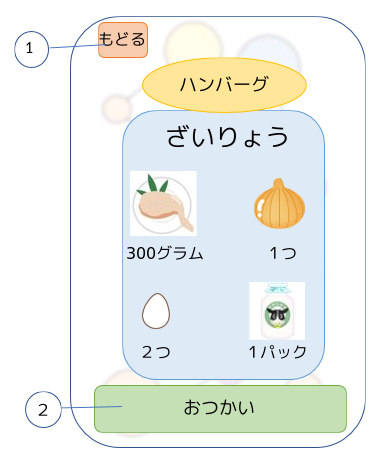
\includegraphics {material.png}}
    \caption {材料画面}
    \label{material}
    \end{center}
\end{figure}

\begin{enumerate}
  \renewcommand{\labelenumi}{\textcircled{\scriptsize \theenumi}}
\item もどるボタン\\
  材料画面(図\ref{material})のもどるボタンをタップするとおつかい画面(図\ref{otukai1})にもどります。
\item おつかいボタン\\
 おつかいのボタンをタップするとお店の画面(図\ref{shop})へ遷移します
\end{enumerate}

\begin{figure}[H]
    \begin{center}
    \resizebox{8cm}{!}{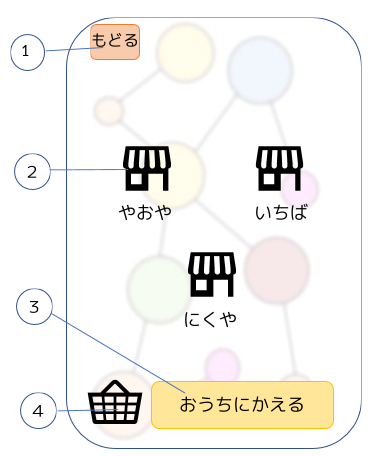
\includegraphics {shop.png}}
    \caption {お店}
    \label{shop}
    \end{center}
\end{figure}

\begin{enumerate}
  \renewcommand{\labelenumi}{\textcircled{\scriptsize \theenumi}}
\item もどるボタン\\
  お店画面(図\ref{shop})のもどるボタンをタップすると食材画面(図\ref{material})にもどります。
\item お店のイラストボタン\\
  お店のイラストボタンをタップするとお店に置いている食材画面(図\ref{shop_material})へ遷移します。
\item かえるボタン\\
  おうちにかえるをタップするとおうち画面(図\ref{myhome})へ遷移します。
\item かごのイラスト\\
  かごのイラストをタップすると持っている材料を確認することができます。
\end{enumerate}

\begin{figure}[H]
    \begin{center}
    \resizebox{8cm}{!}{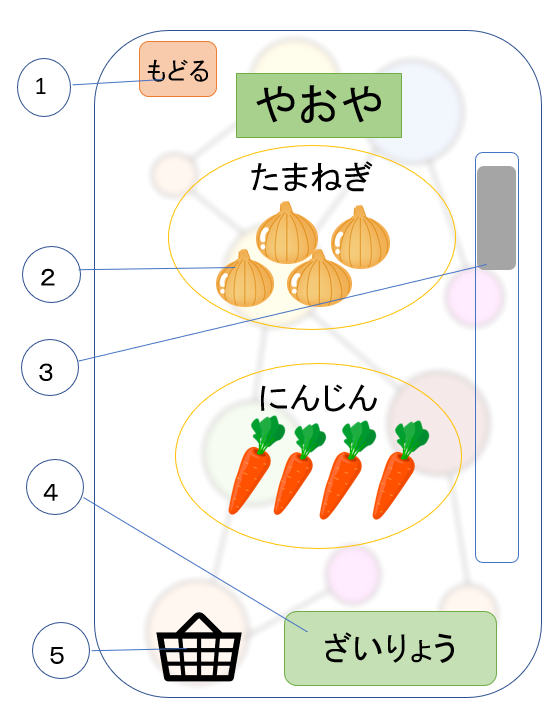
\includegraphics {shop_material.png}}
    \caption {食材画面}
    \label{shop_material}
    \end{center}
\end{figure}

\begin{enumerate}
  \renewcommand{\labelenumi}{\textcircled{\scriptsize \theenumi}}
\item もどるボタン\\
  食材画面(図\ref{shop_material})のもどるボタンをタップするとお店画面(図\ref{shop})にもどります。
\item 食材のイラストボタン\\
  食材のイラストボタンをタップすることで材料の中にタップした食材が1つずつ格納されます。
\item スクロール\\
  スクロールすることでその他の食材を閲覧できます。
\item ざいりょう\\
  ざいりょうをタップすると作りたい料理の材料を確認できます。
\item かごのイラスト\\
  かごのイラストをタップすると持っている材料を確認することができます。
\end{enumerate}

図\ref{myhome}はおうち画面を示します。\\

\begin{figure}[H]
    \begin{center}
    \resizebox{8cm}{!}{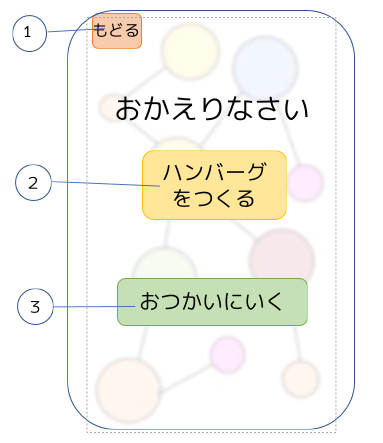
\includegraphics {go_home.png}}
    \caption {おうち画面}
    \label{myhome}
    \end{center}
\end{figure}
\begin{figure}[H]
    \begin{center}
    \resizebox{8cm}{!}{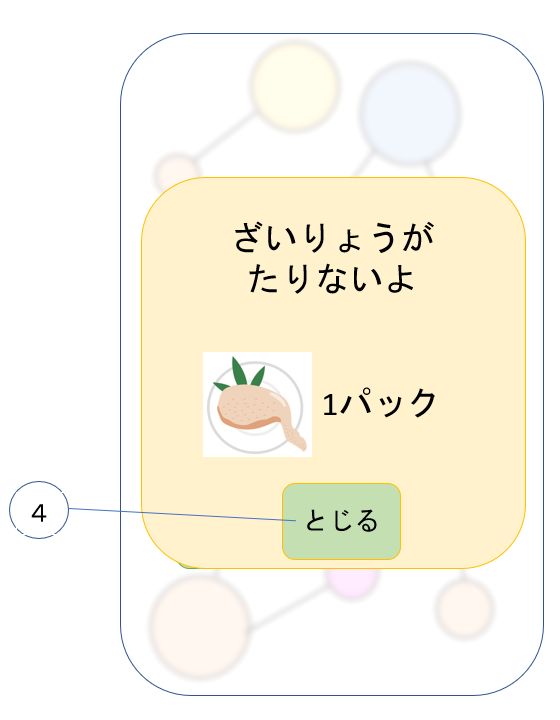
\includegraphics {lack.png}}
    \caption {材料が足りない場合}
    \label{otukai6}
    \end{center}
\end{figure}

\begin{enumerate}
  \renewcommand{\labelenumi}{\textcircled{\scriptsize \theenumi}}
\item もどるボタン\\
  おうち画面(図\ref{myhome})のもどるボタンをタップするとお店画面(図\ref{shop})にもどります。
\item つくるボタン\\
  材料が揃っている場合、おうち画面(図\ref{myhome})のつくるボタンをタップするとできあがり画面(図\ref{completion})へ遷移します。材料が揃っていない場合、図\ref{otukai6}のように「材料が足りないよ」と表示されます。
\item とじるボタン\\
  図\ref{otukai6}の閉じるボタンをタップするとおうち画面(図\ref{myhome})へ遷移します。
\item おつかい\\
  おうち画面(図\ref{myhome})のおつかいにいくをタップするとお店の画面(図\ref{shop})遷移します。
\end{enumerate}

\begin{figure}[H]
    \begin{center}
    \resizebox{8cm}{!}{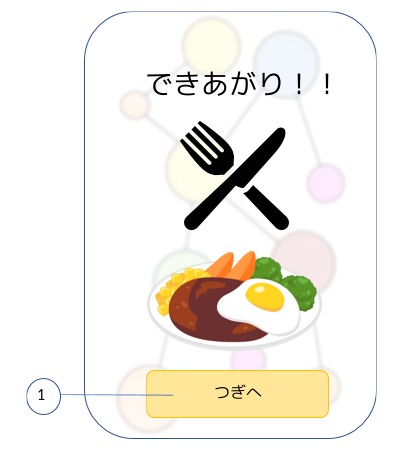
\includegraphics {completion.png}}
    \caption {できあがり画面}
    \label{completion}
    \end{center}
\end{figure}

\begin{enumerate}
  \renewcommand{\labelenumi}{\textcircled{\scriptsize \theenumi}}
\item つぎへ\\
  つぎへをタップすることでおつかいのホーム画面に遷移します。
\end{enumerate}


% 成長記録%
\newpage
\subsection{成長記録}
図\ref{Grow}に、成長記録起動時の画面を示します。
成長記録は、自分の撮影した子どもの写真やゲームの記録を保存し、閲覧及び共有することができます。

\begin{figure}[H]
    \begin{center}
    \resizebox{8cm}{!}{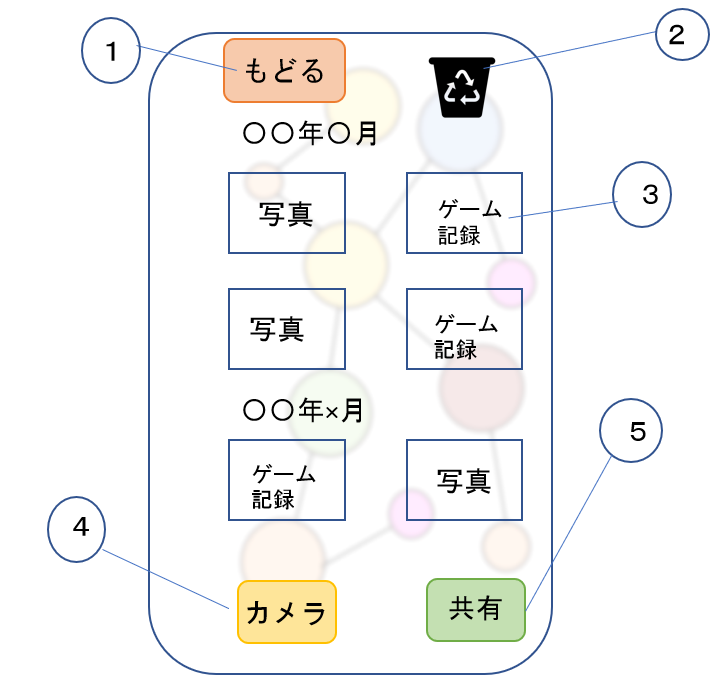
\includegraphics {Albam1.png}}
    \caption {成長記録の画面}
    \label{Grow}
    \end{center}
\end{figure}

\begin{enumerate}
  \renewcommand{\labelenumi}{\textcircled{\scriptsize \theenumi}}
  \item 写真及びゲーム記録\\
       撮影した写真やゲームの記録を閲覧することができます。各写真や記録をタップすると拡大して表示され、保存は月ごとにされていきます。また、メモを残すこともできます。
  \item カメラボタン\\
        撮影したいときに使用するボタンです。ボタンを押すと外部のカメラアプリを起動し写真を撮影することができます。
  \item 共有ボタン\\
        写真やゲームの記録を共有したい時に使用するボタンです。ボタンを押すと外部アプリ(Twitter)を起動し共有することができます。
\end{enumerate}

\newpage
\subsubsection{アルバム画面}
写真をタップしたときに拡大表示される画面(図\ref{Albam})に推移します。
写真や記録は拡大して表示されます。また、共有ボタンもありここから外部アプリ(Twitter)を起動し共有することができます。

\begin{figure}[H]
    \begin{center}
    \resizebox{8cm}{!}{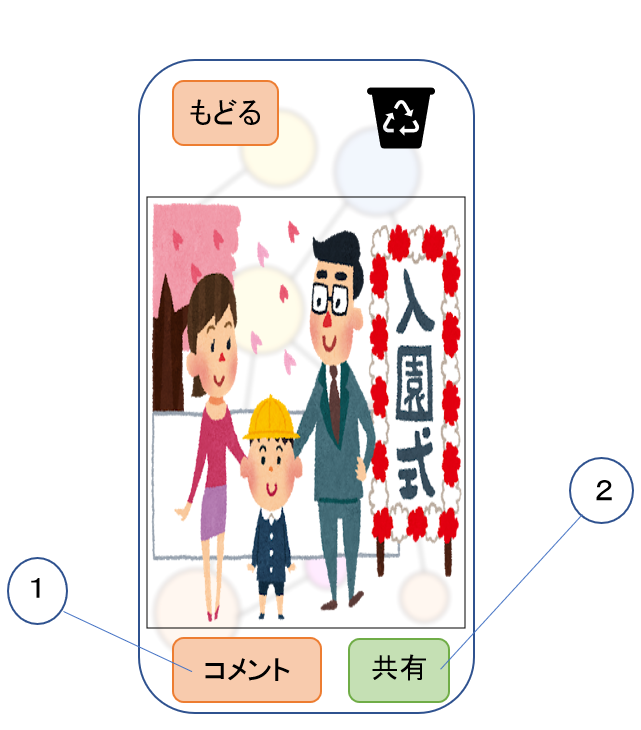
\includegraphics {Albam2.png}}
    \caption {アルバム画面}
    \label{Albam}
    \end{center}
\end{figure}

アルバムに保存された写真や記録にはコメントボタンを押すことによりコメント入力画面(図\ref{Comment})に推移し、コメントを残すことができます。

\begin{figure}[H]
    \begin{center}
    \resizebox{8cm}{!}{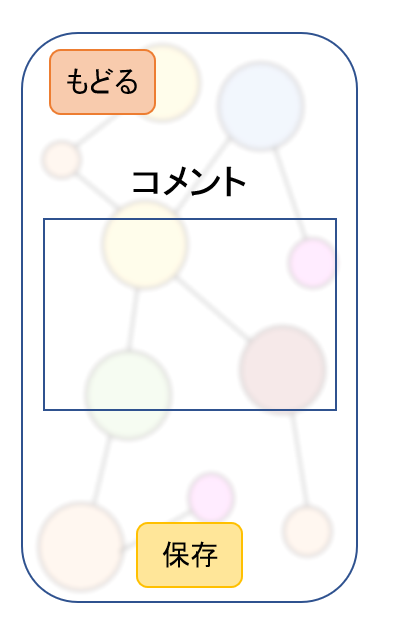
\includegraphics {comment.png}}
    \caption {コメント入力画面}
    \label{Comment}
    \end{center}
\end{figure}

\subsubsection{カメラ}
カメラボタンを押すことにより外部カメラ(図\ref{Camera})を起動します。
カメラを使用して撮影するときに使用されます。ここで撮影された写真はアルバムとして保存され図\ref{Albam}のように閲覧、共有することができます。


\begin{figure}[H]
    \begin{center}
    \resizebox{8cm}{!}{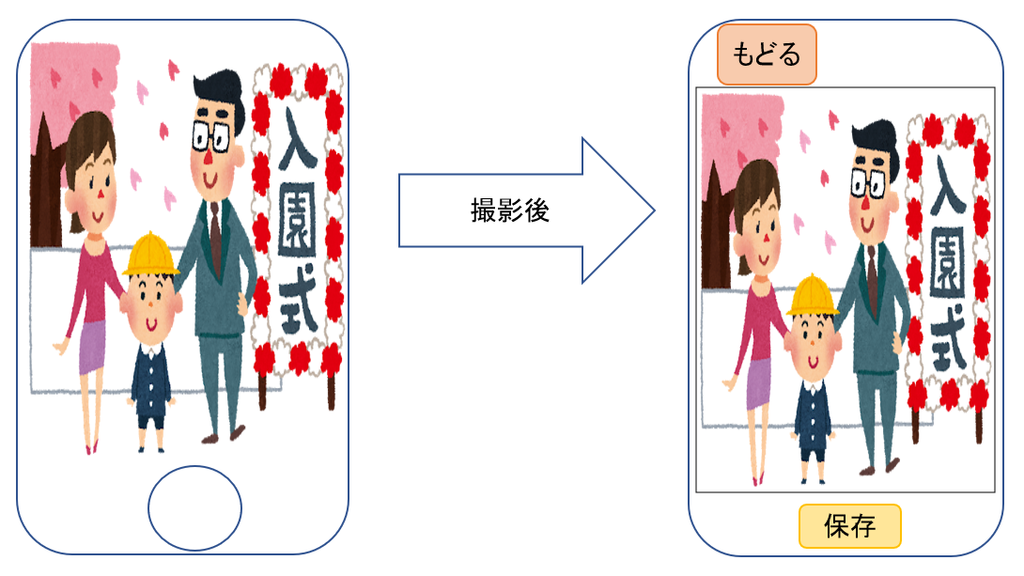
\includegraphics {Camera.png}}
    \caption {カメラ画面}
    \label{Camera}
    \end{center}
\end{figure}


\subsubsection{共有}
写真や記録を他社に共有したいときに使用されます。共有は外部アプリであるTwitterで行われます。共有するためには図\ref{Grow}と図\ref{Albam}についている共有ボタンを押すことで起動することができます。

%質問箱%
\subsubsection{子育て窓口}
図\ref{honjo_CR_Window}に、子育て窓口の画面を示します。
子育てにおける不安・疑問を、検索や投稿を行うことによって解決するために使用されます。

図\ref{honjo_CR_Window}に示す番号と対応させる形式で、以下にその役割を示します。

\begin{figure}[H]
    \begin{center}
    \resizebox{8cm}{!}{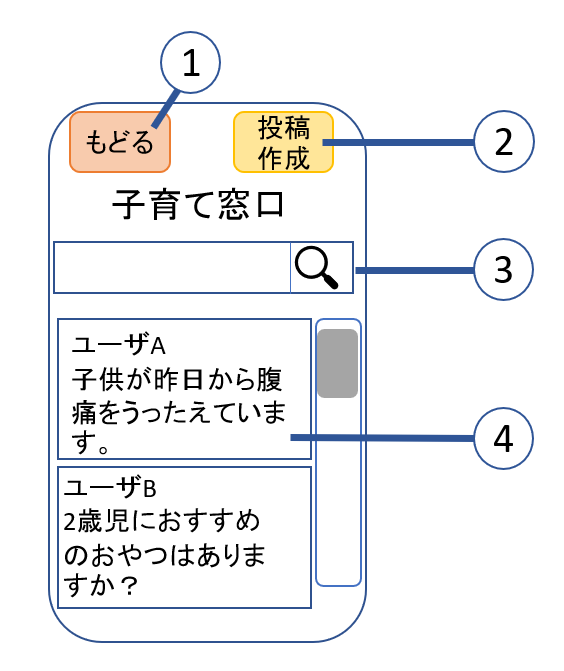
\includegraphics {honjo_CR_Window.png}}
    \caption {子育て窓口の画面}
    \label{honjo_CR_Window}
    \end{center}
\end{figure}

\begin{enumerate}
  \renewcommand{\labelenumi}{\textcircled{\scriptsize \theenumi}}
  \item 戻るボタン\\
        タップすると、メインメニュー画面(図\ref{honjo_main})へ遷移するボタンです。
  \item 質問投稿作成ボタン\\
        質問投稿をしたい時に押すボタンです。ペンのマークをタップすると、質問を行うための投稿画面(図\ref{honjo_CR_Contribution})へ遷移します。
  \item 質問の検索欄\\
        ユーザが子育て窓口内に投稿されたものを検索するために使用します。矩形領域をタップするとキーボードが開き、入力することが可能になります。
  \item 質問の一覧表示\\
        子育て窓口に投稿された質問が一覧表示されます。質問が書かれている矩形領域をタップすると質問の詳細画面(図\ref{honjo_CR_Answer})へ遷移します。
\end{enumerate}

\subsubsection{質問の詳細画面}
図\ref{honjo_CR_Answer}に、質問の詳細画面を示します。
質問の詳細を閲覧、またその質問に対して回答を行うために使用されます。

図\ref{honjo_CR_Answer}に示す番号と対応させる形式で、以下にその役割を示します。

\begin{figure}[H]
    \begin{center}
    \resizebox{8cm}{!}{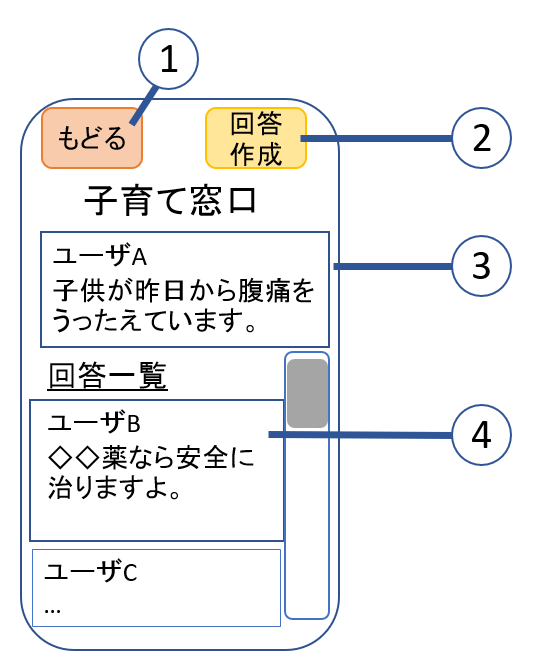
\includegraphics {honjo_CR_Answer.png}}
    \caption {質問の詳細画面}
    \label{honjo_CR_Answer}
    \end{center}
\end{figure}

\begin{enumerate}
  \renewcommand{\labelenumi}{\textcircled{\scriptsize \theenumi}}
  \item 戻るボタン\\
        タップすると、子育て窓口の画面へ遷移するボタンです。
  \item 回答ボタン\\
        この質問に対する回答を作成するためのボタンです。タップすると回答作成画面(図\ref{honjo_CR_CreateAnswer})へ遷移します。
  \item 質問内容\\
        質問内容の全文を表示します。
  \item 回答内容\\
        回答内容の全文を表示します。複数回答がある場合は下にスクロールすることで閲覧が可能になります。
\end{enumerate}

\newpage
\subsubsection{回答作成画面}
図\ref{honjo_CR_CreateAnswer}に、回答の作成画面を示します。
ある質問に対する回答を行うために使用されます。

図\ref{honjo_CR_CreateAnswer}に示す番号と対応させる形式で、以下にその役割を示します。

\begin{figure}[H]
    \begin{center}
    \resizebox{8cm}{!}{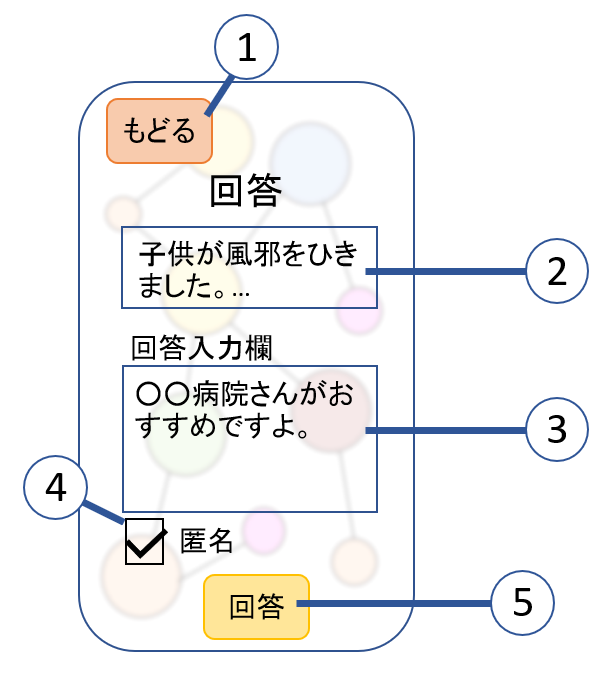
\includegraphics {honjo_CR_CreateAnswer.png}}
    \caption {回答作成画面}
    \label{honjo_CR_CreateAnswer}
    \end{center}
\end{figure}

\begin{enumerate}
  \renewcommand{\labelenumi}{\textcircled{\scriptsize \theenumi}}
  \item 戻るボタン\\
        タップすると、質問の詳細画面(図\ref{honjo_CR_Answer})へ遷移するボタンです。
  \item 質問内容\\
        質問内容の全文を表示します。
  \item 回答内容の入力欄\\
        ユーザが回答内容を入力するための欄です。矩形領域をタップするとキーボードが開き、入力することが可能になります。
  \item 匿名チェックボックス\\
        チェックボックスをタップして、チェックが入ると、匿名で回答を投稿することが出来ます。
  \item 回答投稿ボタン\\
        回答を入力欄に書き終えて投稿をしたい時に押すボタンです。回答投稿完了画面(図\ref{honjo_CR_CompleteAnswer})へ遷移します。
\end{enumerate}

\newpage
\subsubsection{回答投稿完了画面}
図\ref{honjo_CR_CompleteAnswer}に、質問の投稿完了画面を示します。
質問の投稿が正常に完了したことを通知するために使用されます。

図\ref{honjo_CR_CompleteAnswer}に示す番号と対応させる形式で、以下にその役割を示します。

\begin{figure}[H]
    \begin{center}
    \resizebox{8cm}{!}{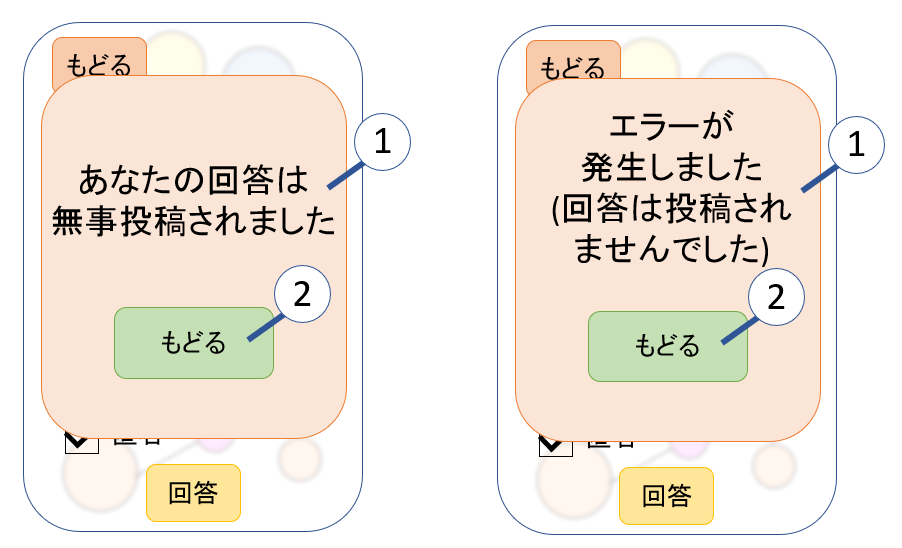
\includegraphics {honjo_CR_CompleteAnswer.png}}
    \caption {回答投稿完了画面}
    \label{honjo_CR_CompleteAnswer}
    \end{center}
\end{figure}

\begin{enumerate}
  \renewcommand{\labelenumi}{\textcircled{\scriptsize \theenumi}}
  \item ステータス\\
        ユーザの回答投稿が正常に完了したかを通知します。
  \item 戻るボタン\\
        子育て窓口の画面(図\ref{honjo_CR_Window})へ遷移するためのボタンです。
\end{enumerate}

\newpage
\subsubsection{質問投稿画面}
図\ref{honjo_CR_Contribution}に、質問の投稿画面を示します。
質問の投稿を行うために使用されます。

図\ref{honjo_CR_Contribution}に示す番号と対応させる形式で、以下にその役割を示します。

\begin{figure}[H]
    \begin{center}
    \resizebox{8cm}{!}{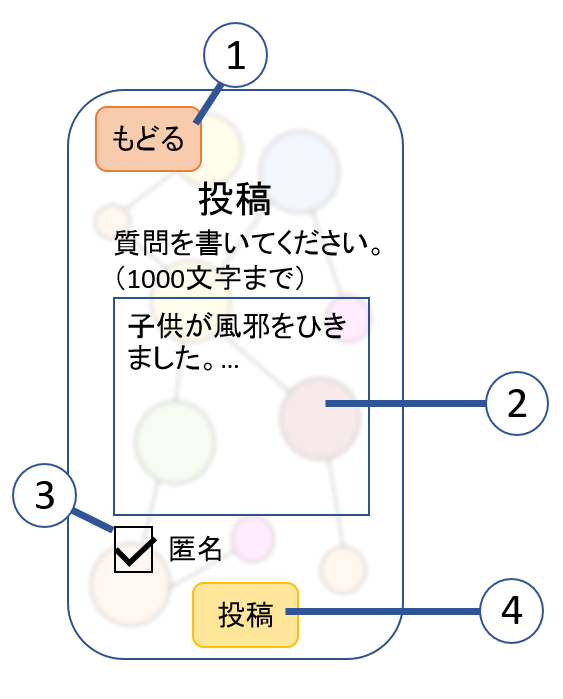
\includegraphics {honjo_CR_Contribution.png}}
    \caption {質問投稿画面}
    \label{honjo_CR_Contribution}
    \end{center}
\end{figure}

\begin{enumerate}
  \renewcommand{\labelenumi}{\textcircled{\scriptsize \theenumi}}
  \item 戻るボタン\\
        タップすると、子育て窓口の画面(図\ref{honjo_CR_Window})へ遷移するボタンです。
  \item 質問内容の入力欄\\
        ユーザが質問の内容を書き込むための欄です。矩形領域をタップするとキーボードが開き、入力することが可能になります。
  \item 匿名チェックボックス\\
        チェックボックスをタップして、チェックが入ると、匿名で回答を投稿することが出来ます。
  \item 投稿ボタン\\
        質問を入力欄に書き終えて投稿をしたい時に押すボタンです。質問投稿完了画面(図\ref{honjo_CR_CompleteContribution})へ遷移します。
\end{enumerate}

\newpage
\subsubsection{質問投稿完了画面}
図\ref{honjo_CR_CompleteContribution}に、質問の投稿完了画面を示します。
質問の投稿が正常に完了したことを通知するために使用されます。

図\ref{honjo_CR_CompleteContribution}に示す番号と対応させる形式で、以下にその役割を示します。

\begin{figure}[H]
    \begin{center}
    \resizebox{8cm}{!}{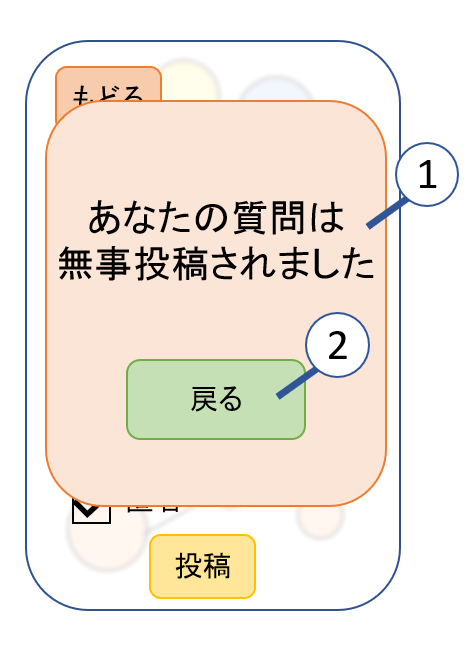
\includegraphics {honjo_CR_CompleteContribution.png}}
    \caption {質問投稿完了画面}
    \label{honjo_CR_CompleteContribution}
    \end{center}
\end{figure}

\begin{enumerate}
  \renewcommand{\labelenumi}{\textcircled{\scriptsize \theenumi}}
  \item ステータス\\
        ユーザの質問投稿が正常に完了したかを通知します。
  \item 戻るボタン\\
        子育て窓口の画面(図\ref{honjo_CR_Window})へ遷移するためのボタンです。
\end{enumerate}

%変更・問い合わせ%
\newpage
\subsection{設定}
図\ref{configuration}は設定画面を示します。\\
設定では、管理者への問い合わせやアカウントの設定をすることができます。

\begin{figure}[H]
    \begin{center}
    \resizebox{8cm}{!}{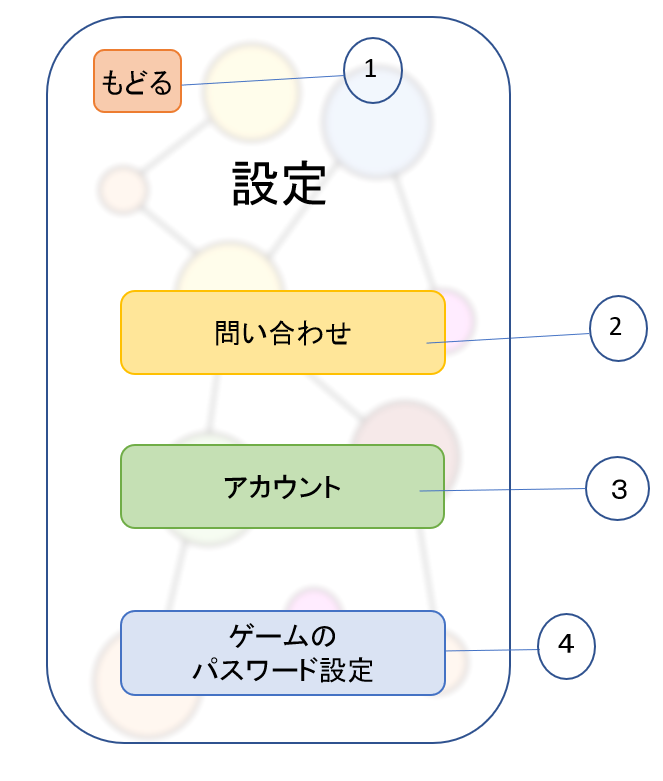
\includegraphics {configuration.png}}
    \caption {設定画面}
    \label{configuration}
    \end{center}
\end{figure}

\begin{enumerate}
  \renewcommand{\labelenumi}{\textcircled{\scriptsize \theenumi}}
\item 問い合わせ\\
  問い合わせをタップすることで問い合わせのメールアドレスと問い合わせに必要な情報を記載したページ(図\ref{inquiry})に遷移します。
\item アカウント\\
  アカウントをタップすると変更と削除の画面(図\ref{account})に遷移します。
\end{enumerate}

\begin{figure}[H]
    \begin{center}
    \resizebox{8cm}{!}{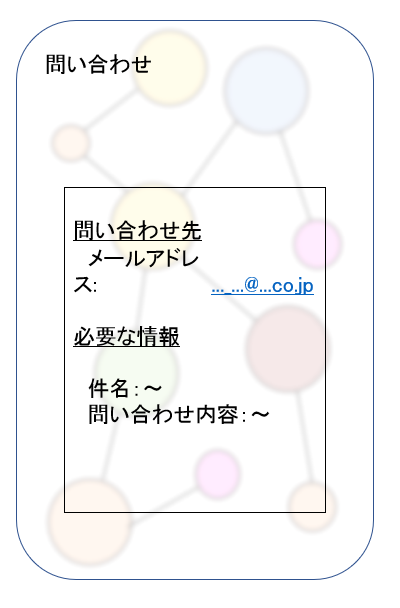
\includegraphics {inquiry.png}}
    \caption {問い合わせ}
    \label{inquiry}
    \end{center}
\end{figure}

\newpage
\subsubsection{アカウント}
図\ref{account}はアカウントの設定画面を示します。\\
アカウントの設定ではアカウントの変更と削除ができます。

\begin{figure}[H]
    \begin{center}
    \resizebox{8cm}{!}{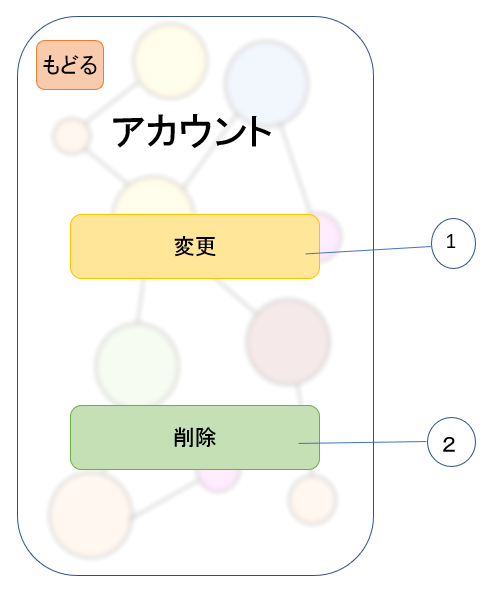
\includegraphics {account.png}}
    \caption {アカウント}
    \label{account}
    \end{center}
\end{figure}

\begin{enumerate}
  \renewcommand{\labelenumi}{\textcircled{\scriptsize \theenumi}}
\item 変更\\
  変更をタップするとニックネームと地域の設定画面(図\ref{change})に遷移します。
\item 削除\\
  削除をタップすると削除をするか確認する画面(図\ref{delete})に遷移します。
\end{enumerate}

\newpage
\subsubsection{削除}
図\ref{delete}はアカウントの削除画面を示します。\\

\begin{figure}[H]
    \begin{center}
    \resizebox{8cm}{!}{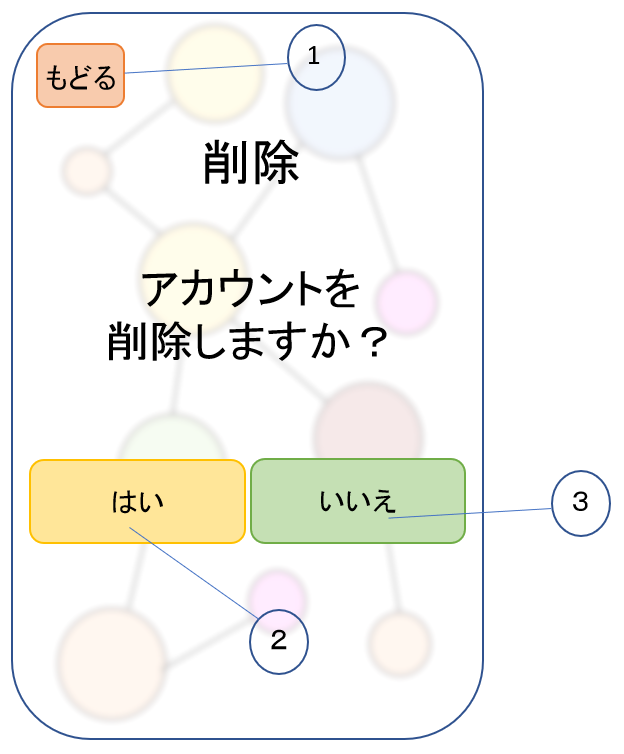
\includegraphics {delete.png}}
    \caption {確認}
    \label{delete}
    \end{center}
\end{figure}

\begin{enumerate}
  \renewcommand{\labelenumi}{\textcircled{\scriptsize \theenumi}}
\item はい\\
  はいをタップすると削除が完了し、完了画面(図\ref{check})へ遷移します。
\item いいえ\\
  いいえをタップするとアカウントの設定画面(図\ref{account})に遷移します。
\end{enumerate}

\begin{figure}[H]
    \begin{center}
    \resizebox{8cm}{!}{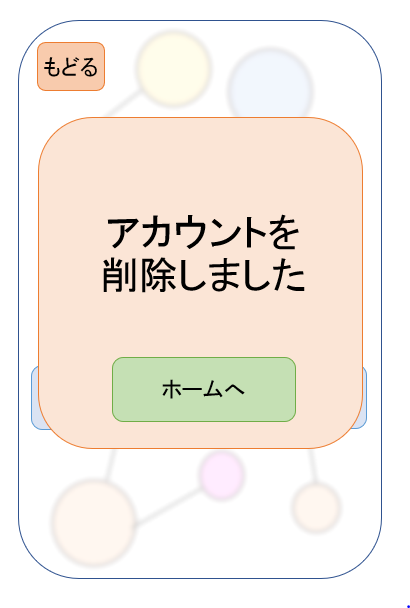
\includegraphics {check.png}}
    \caption {完了}
    \label{check}
    \end{center}
\end{figure}

\newpage
\subsubsection{変更}
図\ref{change}はアカウントの変更画面を示します。\\
変更画面では、ニックネームと地域の変更ができます。

\begin{figure}[H]
  \begin{center}
    \resizebox{8cm}{!}{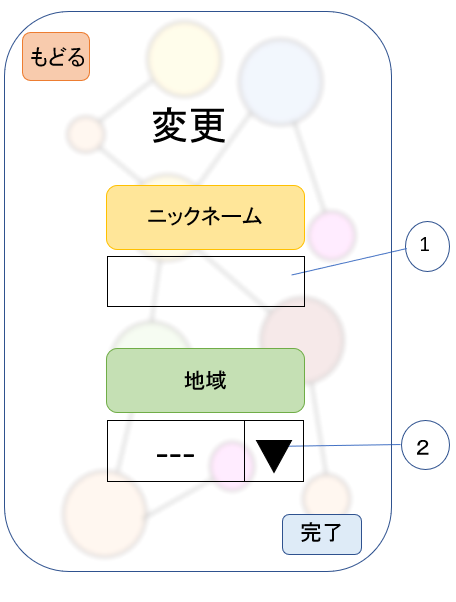
\includegraphics {change.png}}
    \caption {変更}
    \label{change}
  \end{center}
\end{figure}

\begin{enumerate}
  \renewcommand{\labelenumi}{\textcircled{\scriptsize \theenumi}}
\item ニックネーム\\
  ニックネームをタップするとキーボードが開き、入力することが可能になります。
\item 地域\\
  地域をタップすると都道府県の一覧が表示され、選択することができます。
\end{enumerate}

変更後、完了ボタンをタップすることで変更が完了します。

\newpage
\section{データテーブル設計}

以下に本システムで用いるデータテーブルを示します。\\
表\ref{tbl: user}はユーザー情報を示しており、親の情報を格納しています。\\

\begin{table}[H]
    \caption{ユーザー情報}
    \label{tbl: user}
    \begin{center}
        \begin{tabular}{|c|c|c|c|c|} \hline
            属性 & データ型 & データ長 & SQLite & key:Table名\\ \hline \hline
            UserID & 半角英数字型 & 6文字固定長 & TEXT & PK\\ \hline
            Name & 全角文字型 & 10文字可変長 & TEXT & \\ \hline
            Area & 全角文字型 & 5文字可変長 & TEXT & \\ \hline
        \end{tabular}
    \end{center}
\end{table}


表\ref{tbl: question}~表\ref{tbl: date}では、質問箱に関するデータを示しています。表\ref{tbl: question}では質問と質問者の関連付けを、表\ref{tbl: answer}では回答と回答者の関連付けを行い、質問と回答の管理を行っています。\\
また、表\ref{tbl: qcontents}では質問内容を、表\ref{tbl: acontents}では回答内容を、表\ref{tbl: date}では日付の管理を行っています。\\
\begin{table}[H]
    \caption{質問}
    \label{tbl: question}
    \begin{center}
        \begin{tabular}{|c|c|c|c|c|} \hline
            属性 & データ型 & データ長 & SQLite & key:Table名\\ \hline \hline
            QID & 半角英数字型 & 8文字固定長 & TEXT & PK\\ \hline
            UserID & 半角英数字型 & 6文字固定長 & TEXT & FK:親ユーザー情報\\ \hline
            QcontentsID & 半角英数字型 & 10文字固定長 & TEXT & FK:質問内容\\ \hline
            DateID & 半角英数字型 & 8文字固定長 & TEXT & FK:日付\\ \hline
        \end{tabular}
    \end{center}
\end{table}

\begin{table}[H]
    \caption{回答}
    \label{tbl: answer}
    \begin{center}
        \begin{tabular}{|c|c|c|c|c|} \hline
            属性 & データ型 & データ長 & SQLite & key:Table名\\ \hline \hline
            AID & 半角英数字型 & 8文字固定長 & TEXT & PK\\ \hline
            QID & 半角英数字型 & 8文字固定長 & TEXT & FK:質問\\ \hline
            UserID & 半角英数字型 & 6文字固定長 & TEXT & FK:親ユーザー情報\\ \hline
            AcontentsID & 半角英数字型 & 10文字固定長 & TEXT & FK:回答内容\\ \hline
            DateID & 半角英数字型 & 8文字固定長 & TEXT & FK:日付\\ \hline
        \end{tabular}
    \end{center}
\end{table}

\begin{table}[H]
    \caption{質問内容}
    \label{tbl: qcontents}
    \begin{center}
        \begin{tabular}{|c|c|c|c|c|} \hline
           属性 & データ型 & データ長 & SQLite & key:Table名\\ \hline \hline
            QcontentsID & 半角英数字型 & 10文字固定長 & TEXT & PK\\ \hline
            Qcontents & 全角文字型 & 100文字可変長 & TEXT & \\ \hline
        \end{tabular}
    \end{center}
\end{table}


\begin{table}[H]
    \caption{回答内容}
    \label{tbl: acontents}
    \begin{center}
        \begin{tabular}{|c|c|c|c|c|} \hline
            属性 & データ型 & データ長 & SQLite & key:Table名\\ \hline \hline
            AcontentsID & 半角英数字型 & 10文字固定長 & TEXT & PK\\ \hline
            Acontents & 全角文字型 & 100文字可変長 & TEXT & \\ \hline
        \end{tabular}
    \end{center}
\end{table}

\begin{table}[H]
    \caption{日付}
    \label{tbl: date}
    \begin{center}
        \begin{tabular}{|c|c|c|c|c|} \hline
            属性 & データ型 & データ長 & SQLite & key:Table名\\ \hline \hline
            DateID & 半角英数字型 & 8文字固定長 & TEXT & PK\\ \hline
            Date & 日付型 & 20文字固定長 & NUMERIC & \\ \hline
        \end{tabular}
    \end{center}
\end{table}


また、表\ref{tbl: datatable}に上記のデータテーブルに対する操作を示します。ユーザー情報はユーザー側と管理者側の両方で編集できるようにします。質問と回答のテーブルはユーザーが作成を行い、削除は管理者側が行えるようにします。質問内容と回答内容は内容を修正できるようにユーザーが更新できるようにしておきます。日付は自動で保存されるので参照のみできるようにします。

\begin{table}[H]
    \caption{各種データテーブルに対する操作}
    \label{tbl: datatable}
    \begin{center}
        \begin{tabular}{|l||c|c|c|c||c|c|c|c|} \hline
             & \multicolumn{4}{|c||}{アプリケーション} & \multicolumn{4}{|c|}{管理画面}\\ \hline
            データテーブル & \multicolumn{1}{|l|}{作成} & \multicolumn{1}{|l|}{参照} & \multicolumn{1}{|l|}{更新} & \multicolumn{1}{|l||}{削除} & \multicolumn{1}{|l|}{作成} & \multicolumn{1}{|l|}{参照} & \multicolumn{1}{|l|}{更新} & \multicolumn{1}{|l|}{削除}\\ \hline \hline
            ユーザー情報 & 〇 & 〇 & 〇 & 〇 & 〇 & 〇 & 〇 & 〇\\ \hline
            質問 & 〇 & 〇 &  &  & 〇 & 〇 & 〇 & 〇\\ \hline
            質問内容 & 〇 & 〇 & 〇 &  & 〇 & 〇 & 〇 & 〇\\ \hline
            回答 & 〇 & 〇 &  &  & 〇 & 〇 & 〇 & 〇\\ \hline
            回答内容 & 〇 & 〇 & 〇 &  & 〇 & 〇 & 〇 & 〇\\ \hline
            日付 &  & 〇 &  &  & 〇 & 〇 & 〇 & 〇\\ \hline
        \end{tabular}
    \end{center}
\end{table}


%付録%
\newpage
\appendix
\section{付録}
図\ref{全体}, \ref{成長記録}, \ref{ゲーム}, \ref{SNS}は本システムのユースケース図を示しています。

\begin{figure}[H]
  \begin{center}
    \resizebox{8cm}{!}{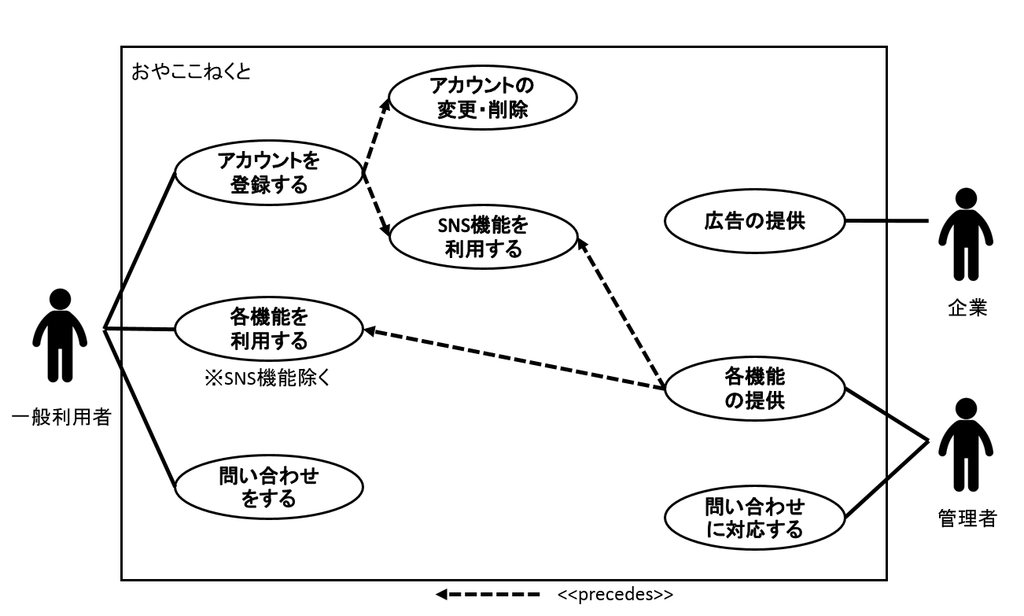
\includegraphics {zentai.png}}
    \caption{システム全体のユースケース図}
    \label{全体}
  \end{center}
\end{figure}

\begin{figure}[H]
  \begin{center}
     \resizebox{8cm}{!}{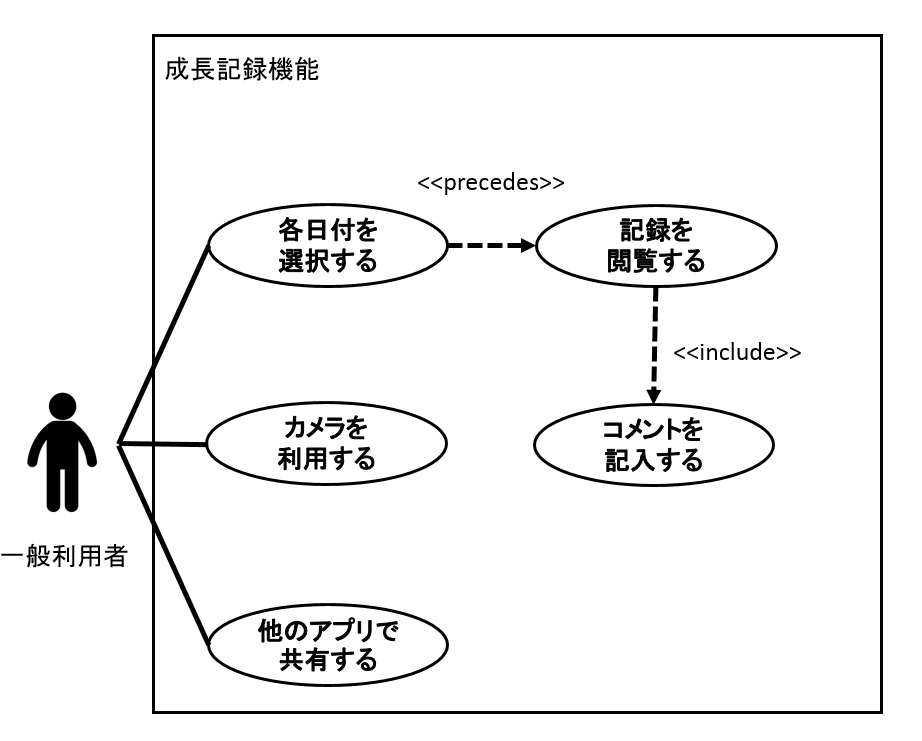
\includegraphics{seithou.png}}
    \caption{成長記録機能のユースケース図}
    \label{成長記録}
  \end{center}
\end{figure}

\begin{figure}[H]
  \begin{center}
     \resizebox{8cm}{!}{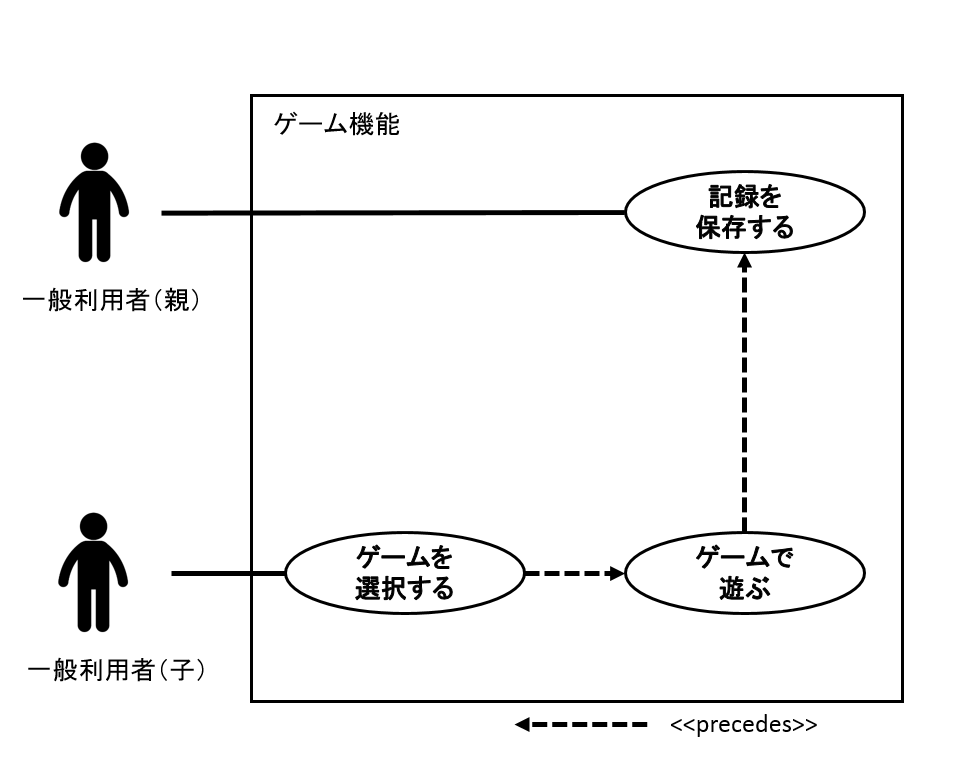
\includegraphics{ugame.png}}
    \caption{ゲーム機能のユースケース図}
    \label{ゲーム}
  \end{center}
\end{figure}

\begin{figure}[H]
  \begin{center}
     \resizebox{8cm}{!}{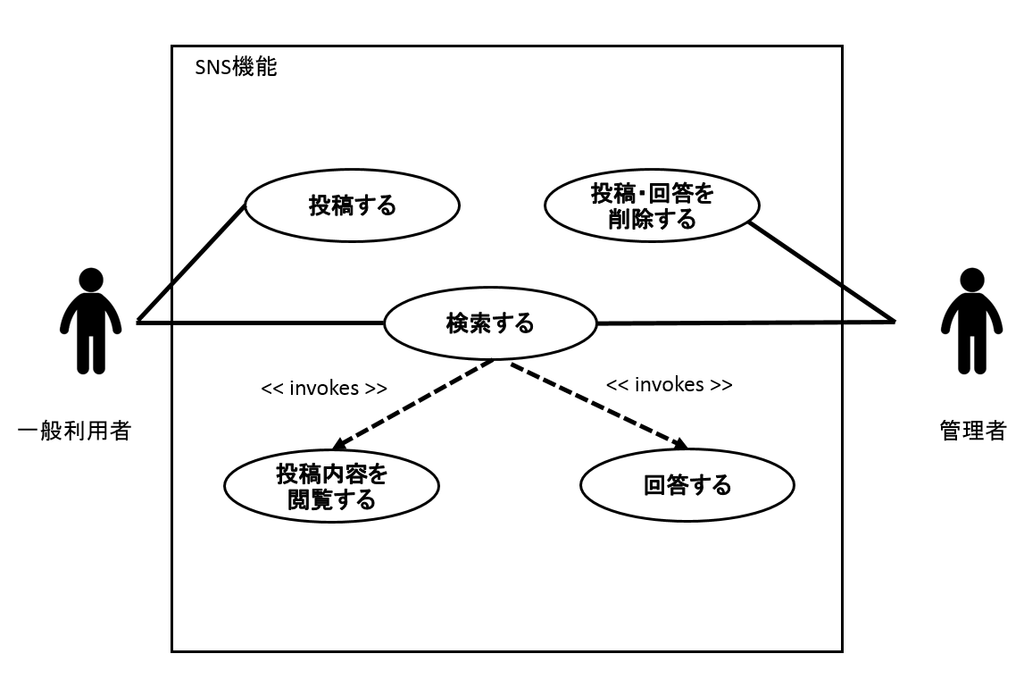
\includegraphics{sns.png}}
    \caption{SNS機能のユースケース図}
    \label{SNS}
  \end{center}
\end{figure}

\end{document}
